\chapter{Problemanalyse}

TODO: Abschnitt neu schreiben

Die Zusammenführung der Arbeit von mehr als einem Entwickler ist ein komplexer und nicht trivialer Vorgang. \\
Viele Teile eines Softwareprojektes beeinflussen andere und häufig werden an Schnittstellen in Programmen Änderungen von mehreren Entwicklern vorgenommen. \\
Es muss sichergestellt werden, dass die Änderungen zusammengeführt werden können und dass das Ergebnis syntaktisch und semantisch korrekt ist, sowie den Anforderungen entspricht.

Während die syntaktische und semantische Validierung klassische Themen der theoretischen Informatik sind, erfordert die Erhebung und Aufbereitung von Anforderungen eine ganz eigene Betrachtung durch ein konkretes Anforderungsmanagement.

Gerade wenn die Software einen gewissen Umfang übersteigt, ist daher ein solides Anforderungsmanagement essenziell. Zudem müssen Mechanismen geschaffen werden, um sicherzustellen, dass diese Anforderungen über die komplette Laufzeit der Software erfüllt bleiben. 

Leider sieht die Realität in der Softwareentwicklung nicht selten anders aus. Fehlende, nicht dokumentierte oder veraltet Anforderungen sind keine Seltenheit.\\
Ebenso sind lange Zeitintervalle in denen sich Teile der Software in keinem lauffähigen oder einem fehlerbehaftetem Zustand befinden häufig anzutreffen.

Fehlende Anforderungen und fehlerhafte Umsetzungen werden häufig erst zum Zeitpunkt des Testes - oder schlimmer - zum Zeitpunkt der Auslieferung offenbart.

Die Gründe für diese Schwierigkeiten sind häufig in kein homogenes Bild zu bringen. Vielmehr tragen verschiedene Faktoren dazu bei, die erst in der Kombination zu erheblichen Problemen führen können.

\section{Vorgehensmodelle}

Um komplexe Software in einer strukturierten und definierten Herangehensweise zu erstellen, wurden ausführlich
beschriebene und wohl definierte Vorgehensmodelle erarbeitet. Deren Ziel ist es eine klare Schrittfolge mit 
eindeutigen Zielstellungen vorzugeben. Diese Schritte gliedern den komplizierten und komplexen Entwicklungsprozess 
in klar abgegrenzte und bewertbare Abschnitte. 

Die bekanntesten Vorgehensmodelle halten sich an eine klare Folge aus Planungs-,\\ Konzeptions-, Implementierungs-, 
Test- und Abnahmephase. Durch die klare Trennung der Phasen werden diese Modelle auch statische Vorgehensmodelle genannt.
Beispiele sind hier das Wasserfallmodell[quote Wasserfallmodell] und das V-Modell[quote V-Modell]. Insbesondere in
Bereichen mit hohen Sicherheitsanforderungen und einer starken Bindung an bürokratische Strukturen wird auch heute noch
das V-Modell erfolgreich eingesetzt[quote Referenz Bund].

Mit der Komplexität einer Softwareanwendung steigt ihr Umsetzungsaufwand. Dieser zusätzliche Aufwand teilt sich in
statischen Vorgehensmodellen in die einzelnen Phasen auf. Bei besonders umfangreichen Softwareprojekten entsteht daher
eine signifikante zeitliche Diskrepanz zwischen den Phasen der Anforderungsaufnahme und deren Umsetzung. 
Zudem ist der Vorgang der Anforderungsaufnahme ohnehin schwierig ist und kann nur schwer auf Vollständigkeit geprüft
werden. Diese beiden Faktoren erhöhen das Risiko eine fehlerhafte Softwareanwendung zu erstellen. Aus der hohen Dauer der
einzelnen Phasen ergibt sich zudem eine hohe Reaktionszeit um fehlerhaft umgesetzte Anforderungen zu korrigieren.

Ein Projekt zur Umsetzung einer komplexen Softwareanwendung benötigt ein umfangreiches Risikomanagement, um Folgekosten 
zu verringern.

Um den Aufwand für das Risikomanagement und die Folgekosten zu minimieren entwickelte sich eine alternative
Herangehensweise, welche vor allem Interaktion, Funktionalität, Kundenorientierung und Veränderungsbereitschaft als
wichtig erachtet. Festgehalten im Agilen Manifest[quote manifest] proklamierten viele bekannte und angesehene
Softwareexperten ihren Willen Softwareprojekte grundsätzlich anders zu fokussieren.

Beeinflusst von der Lean-Bewegung aus der Automobil-Fertigungsindustrie\footcite{kent1999} wurden die abgegrenzten Phasen 
in den statischen Vorgehensmodellen in Frage gestellt. Hohe Eigenverantwortung und kurze Kommunikationszyklen sind die 
Basis des neuen Vorgehens.

Die Prinzipien des ``Agilen Manifestes'' stellen hohe Ansprüche an Entwickler und erzwingen ein Umdenken im Umgang mit dem Projektprozess. Während in den statischen Vorgehensmodellen jede Phase eine längere zeitliche Periode einnimmt, so werden diese Phasen in agilen Vorgehen deutlich verkürzt und verschwimmen teilweise. Dadurch werden Kommunikationszyklen verkürzt und Informationsflüsse deutlich beschleunigt.
Durch die schnellere Zyklen sinkt die benötigte Zeit zur Reaktion auf Probleme und Hindernisse. Damit ist es möglich kontinuierlich und zeitnah Verbesserungen für den Entwicklungsprozess und die Softwareanwendung einzubringen. 

Agile Vorgehensmodelle und Techniken aus der Lean-Bewegungen setzen stark auf eine Arbeitseinteilung anhand von Produktmerkmalen(Features)[quote Scrum, quote Kanban]. Der von der agilen Bewegung angestrebte starke Produktfokus und die kurzen Iterationen vereinfachen die Bewertung des Projektprozesses und der verwendeten Hilfsmittel.

Der hohe Fokus auf Produktmerkmale und das Prinzip zur frühen und kontinuierlichen Auslieferung von wertvoller Software\footcite{agile-manifest-principles} helfen die Akzeptanz für die Software zu steigern. Außerdem können falsch interpretierte Anforderungen früher erkannt werden. 

Um die Umsetzung der Anforderungen zu prüfen benötigt es eine Qualitätssicherung. Für komplexe Softwareanforderungen ist die Prüfung der Anforderungen mit sehr hohem Aufwand verbunden, wenn sie manuell ausgeführt wird. Um Anforderungen automatisiert zu prüfen, müssen diese abstrakt formuliert werden. Der damit verbundene Aufwand steigt, wenn sich die Anforderungen häufig ändern. Dies sollte in einer Strategie für die Qualitätssicherung beachtet werden. 

\section{Qualitätssicherung und Softwaretest}

Die Erfüllung der Anforderungen an eine Softwareanwendung sollte durch eine Strategie der Qualitätssicherung sichergestellt sein. Da jede Änderung an der Software die Erfüllung der Anforderungen beeinträchtigen könnte, sollten die Anforderungen nach Änderungen erneut geprüft werden. Da manuelle Prüfungen aufwändig und zeitintensiv sind, sollten sie sich auf wenige Anwendungsszenarien beschränken. Diese Anwendungsszenarien sollten nur schwer oder unzuverlässig durch programmierte Prüfungen abgedeckt werden können.

Programmierte Prüfungen, auch Tests genannt, zu erstellen kann sehr komplex und kompliziert sein. Je nach Softwareanwendung und damit verbundenen Anforderungen, müssen Kompromisse zur Laufzeit, Aussagekraft und Wartbarkeit eines Tests eingegangen werden.
Den jeweiligen Schwerpunkten eines Tests geschuldet, werden Tests auf verschiedenen Abstraktionsebenen der Software ausgeführt. Üblicherweise wird zwischen Akzeptanz-, Funktions-, Integrations- und Unittests unterschieden.[quote softwarequalität]. 

\paragraph{Akzeptanztest}
oder auch Abnahmetests stellen in erster Linie die Erfüllung der definierten Anforderungen sicher. Akzeptanztests werden häufig in der Form von Anwendungsszenarien (Use-Cases) beschrieben. Anwendungsszenarien beschreiben das Zusammenspiel von Systemen, deren Akteuren und Aktionen die zwischen diesen ausgeführt werden. Die Verwendung von technischen Details der Software, wie Datenbankspezifikationen oder konkreten Systemimplementierungen sollten vermieden werden. Nicht nur erhöht es den Wartungsaufwand dieser Tests, es verschiebt auch den Fokus des Tests, weg von den eigentlich zu prüfenden Anforderungen.

\paragraph{Funktions- und Integrationstests}

dienen der Überprüfung von Schnittstellen. Dabei wird das Verhalten der Schnittstelle auf definierte Ein- und Ausgaben geprüft. Der Fokus der Tests liegt darauf unerwartetes Verhalten beim Zusammenspiel mehrere Komponenten auszuschließen.

\paragraph{Unit-Tests}

werden für Objektklassen- und Methodentests verwendet. Das erwartet Verhalten der zu überprüfenden Einheit(Unit) wird mit dem Unit-Test sichergestellt. Zugleich übernimmt er auch eine dokumentarische Funktion. Durch die Initialisierung der Einheit und der Aufruf ihrer Schnittstelle, wird die Intention ihres Autors deutlich.

\section{Automatisierung der Softwareerstellung}

Zur Bereitstellung einer Softwareanwendung werden mehrere Schritte benötigt. Es wird ein konkreter Stand der Softwarequellen benötigt, ein ausführendes System und es muss für eine Kompilierung der Softwarequellen zu dem System gesorgt werden.
Je nach Anforderung und Art der Softwareanwendung entspricht dieser Vorgang einer trivialen Kopie oder einem mehrstufigen, komplexen Vorgang. 

Im Nachfolgenden wird beschrieben wie Software in einen wohldefinierten, funktionalen Zustand gebracht und dieser validiert wird. Dazu wird auf Versionsverwaltungssysteme, Konfigurationsmanagement, die automatisierte Erstellung und deren Test eingegangen.

\subsection{Kodeverwaltung und Versionsverwaltungssysteme}

Programmversionen können bei fast jeder käuflich zu erwerbenden Softwareanwendung unterschieden werden. Potentielle Anwender konnten so bereits vor Erwerb transparent nachvollziehen, wie fortschrittlich die Anwendung war.
Für die Entwicklung ergab sich daraus die Herausforderung Fehlerkorrekturen nach Veröffentlichung der Software, für viele verschiedene Programmversionen bereit zustellen.
Eine nachvollziehbare und leicht zu verwendende Ablage der einzelnen Programmversionen war daher sehr hilfreich.

Die einfachste Form der Ablage ist eine manuelle Kopie der Softwareanwendung. Mit der Weiterentwicklung der Anwendung und dem Entstehen weiterer Programmversionen zeigen sich schnell schwächen dieses Systems. Wenn in einer frühen Programmversion ein Fehler gefunden und behoben wird, sollte dieser auch in allen anderen folgenden Versionen behoben werden. Dadurch entsteht mit dieser einfachen Ablage ein erheblicher Mehraufwand. Fortschrittliche Versionsverwaltungssysteme bieten Möglichkeiten diesen Mehraufwand zu reduzieren.

Ein besonders wichtiges Merkmal eines Versionverwaltungs- oder auch Versionskontrollsystems, ist die Zustandssicherheit. Die Reproduzierbarkeit eines definierten Zustandes der Softwarequellen. Der definierte Zustand der Anwendung ergibt sich aus der Abfolge aller Änderungen, die an der Softwareanwendung vorgenommen wurden, bis zu der jeweiligen Programmversion. 

Als weiteres Merkmal ist die Transparenz aller getätigten Änderungen anzuführen. Wenn mehr als ein Entwickler am Quellcode einer Anwendung arbeitet, ist die Nachvollziehbarkeit aller Änderungen wichtig. 


Schnell geht die Übersicht verloren, welche Änderungen wann, von wem und warum eingebracht wurden. Oftmals sind diese Informationen aber hilfreich um Entscheidungen im Entwicklungsprozess zu treffen.

Über die Entstehung von Versionsverwaltungssysteme[quote Soft.Quali] haben sich vor allem zwei Prinzipien herausgebildet: Zentrale und Dezentrale Versionsverwaltungssysteme. Zwar unterscheiden sich die Versionsverwaltungssysteme auch in anderen Merkmalen, zum Beispiel in der Ablage der Quellen und deren Änderungen, diese Merkmale haben aber nahezu keinen Einfluss auf die Verwendung im Softwareentwicklungsprozess.

Auch wenn heutzutage die dezentralen Versionsverwaltungssystem stark zunehmen, so fällt bei näherer Betrachtung auf, dass diese oft primär als zentrale Versionsverwaltungssysteme verwendet werden.

\paragraph{Zentrale Versionsverwaltungssysteme} folgen dem Prinzip, dass es nur einen zentralen Punkt gibt auf dem alle Versionstände gespeichert werden. Dieses ``single point of truth'' Prinzip sorgt für einen einfachen Kontrollfluss, welcher dafür sorgt, dass alle Partizipierer mit einfachen Mitteln auf den gleichen Versionsständen arbeiten. Damit einhergehend ist eine Übersicht aller Änderungen problemlos möglich.

Nachteil dieser Variante ist häufig der Initialaufwand, da eine zentrale Komponenten bereitgestellt werden muss. Zudem sind zentrale Systeme generell störanfälliger und Probleme betreffen immer alle Teilnehmer gleichzeitig.
Je nach verwendeter Versionierungsstrategie kann es zudem zu einer zentralen Blockade ganzer Bereiche der Softwarequellen kommen, wenn diese für eine exklusive Bearbeitung gesperrt sind.

\paragraph{Dezentrale Versionsverwaltungssysteme} benötigen im Gegensatz keine zentrale Instanz und können problemlos in einem losen Verbund von Einzelsystemen betrieben werden. 
Im Gegensatz zur zentralen Verwendung, existierend dadurch deutlich mehr Zustände, die ohne entsprechende Maßnahmen nicht zu überblicken sind. Dieser Mehraufwand bringt allerdings eine Flexibilität mit sich, welche viele Möglichkeiten bietet um Softwareänderungen zu koordinieren. Änderungen können in ihrer Reihenfolge transparent manipuliert und der Zeitpunkt der Zusammenführung beliebig gewählt werden. 
Im Bereich ``Feature-Branches'' werden Versionierungsstrategien im Detail erläutert.

Ihrer dezentralen Natur geschuldet, sind sie ausfallsicherer als die zentralen Versionsverwaltungssysteme, benötigen allerdings die entsprechenden Informationen und Befugnisse zur Verbindung, um diesen Vorteil nutzen zu können.

\subsection{Konfigurationsverwaltung}
\label{subsec:konfigurationsverwaltung}

Konfigurationsverwaltung ist eine wichtige Basis für die automatisierte Erstellung eines Softwareprojektes. Sie definiert wie alle Artefakte in einem Softwareprojekt orchestriert werden. Im Detail wird dabei Erstellung, Identifikation, Validierung und Ablage geregelt. Neben den Projekteigenen Artefakten müssen aber auch deren Umgebung genau definiert sein. \footcite{humble2010}

Ein lockerer Umgang mit der Konfigurationsverwaltung kann gerade zu Anfangs ohne nennenswerte Folgen einhergehen. Spätestens aber während der Reifung und Alterung eines Softwareprojektes sind Folgen deutlich zu spüren. Gerade wenn sich unbemerkt die Version oder Konfiguration der Software eines Drittanbieters ändert, kann dies zu sehr schwer zu identifizierbaren Problemen führen. In anderen Fällen reicht es allerdings auch, wenn sich die Konfiguration zwischen Entwicklungs- und Produktivumgebung leicht unterscheidet. Auch hier können damit zusammenhängende Fehler unnötig viel Zeit in Anspruch nehmen.

Im Idealfall kann eine vollständige Konfigurationsverwaltung:
\begin{itemize}
\item eine Umgebung bereitstellen, die genau definiert welches Betriebssystem, in welcher Version, installiert ist und welche Anwendungen, mit welcher Konfiguration, darauf liegen
\item auf jeder Umgebung jeden dieser Bestandteile einzeln inkrementell verändern und diese Änderungen auch synchronisiert bereit stellen.
\item alle Änderungen mit Zeitpunkt und Verursacher einfach darstellen
\item Sicherheitsregeln und Konventionen über alle Systeme sicherstellen
\item alle diese Funktionalitäten barrierefrei dem Entwicklungsteam zur Verfügung stellen
\end{itemize}

Alle Forderungen sind sicherlich nicht immer Notwendig, sorgen aber dafür, dass Projekte langfristig, mit geringem Aufwand betreut werden können. Zudem wird deutlich, dass Virtualisierung und Versionsverwaltung[quote cont.deliv] der entsprechenden Komponenten den einhergehenden Aufwand deutlich verringern können.

\subsection{Abhängigkeitsverwaltung}

In der Abhängigkeitsverwaltung werden die Softwareabhängigkeiten der Anwendung beschrieben. In auf  Komponenten basierenden Anwendungen schließt dies die eigenen, interne Abhängigkeiten mit ein. Diese Abhängigkeiten, meist Module genannt, sollen die mit monolithischen Strukturen einhergehenden Nachteile unterbinden. Monolithen leiden häufig unter einer schwachen Softwarearchitektur und entwickeln sich daher entsprechend schlecht weiter. Mögliche Skalierungen des Systems oder ein Austausch von einzelnen Bestandteilen sind mit einem erheblichen Mehraufwand verbunden.

Ist eine Anwendung hingehen auf mehrere Komponenten aufgeteilt, kommen neben den genannten Vorteilen der Skalierbarkeit und Austauschbarkeit, auch Vorteile für das verteilte Arbeiten von Teams. Allerdings führt eine Komponenten basierende Anwendung natürlich auch zu einem organisatorischem Mehraufwand. Dieser Mehraufwand besteht in der Beschreibung der Abhängigkeiten und der Auflösung des damit entstehenden Abhängigkeitsgeflechtes. Übliche Abhängigkeitsverwaltungen verwenden hierzu Versionsnummer aus der Versionsverwaltung, sowie eine Paketbeschreibung in einem eigenen Format. 

Für die automatisierte Erstellung der Softwareanwendung ist es erforderlich, ähnlich wie bereits bei der Versionsverwaltung, ein eindeutiges Abhängigkeitsbild zu beschreiben. Während zum Auflösen der Abhängigkeiten meist mehrdeutige Ausdrücke verwendet werden, die eine Bandbreite an Versionen der Abhängigkeiten erlauben, ist für den Erstellungsvorgang wichtig die konkret verwendeten Versionen zu dokumentieren und mit dem erstellten Produkt auszuliefern. Ähnlich der erwähnten Paketbeschreibung, wird dies mit einer Lock-Datei gesichert.

\subsection{Automatisierte Erstellung und Auslieferung}

Der an sich triviale Schritt, der Erstellung (Build) einer Anwendung, birgt gewisse Tücken. So kann die Ausführung eines komplexen Erstellungsskriptes einen sehr langen Zeitraum in Anspruch nehmen und ein besonders kompliziertes Skript kann die Arbeit damit intransparent gestalten und das Entwicklungsverhalten deutlich benachteiligen. [quote paper] Werden bei einem Erstellungsskript Aspekte der vorangegangen Abschnitte zu Versions-, Konfigurations- und Abhängigkeitsverwaltung nicht berücksichtigt, können zudem inkonsistente und damit nicht wiederholbare Resultate erzeugt werden. Diese können leicht zu schwer oder nicht auffindbaren Fehlern führen.

Ziel bei der Erstellung eines Erstellungsskriptes ist es folglich einen konsistenten und transparenten Ablauf zu befolgen. Dies wird unter anderem durch die korrekte Versionsverwaltung der einzelnen Komponenten, Konfigurationen und Abhängigkeiten erreicht. Mit diesen Informationen können erstellte Produkte, auch ``build artifacts'' oder Artefakte genannt, in einem zentralen Artefakt-Lager abgelegt werden. Dies gewährleistet sowohl einen schnellen Zugriff auf Teilartefakte, als auch einen konsistentes Ergebnis bei der Erstellung der Auslieferung.

Die Auslieferung der Software ist direkt mit der Erstellung verwoben. Bei jeder Auslieferung muss sichergestellt werden, dass Software auf dem entsprechenden Zielsystem auch lauffähig ist und dass sie richtig konfiguriert ist für das Zielsystem. Ein vollständiges Konfigurationsmanagement beschreibt die Systemabhängigkeiten und sorgt folglich für die korrekte Auslieferung der richtigen Artefakte.

Sowohl bei der Erstellung, als auch bei der Auslieferung ist insbesondere auf eine vollständige Beschreibung und die Einhaltung dieser zu achten. Gerade auf Entwicklungssystemen können Abhängigkeiten vorhanden sein, welche zwar für die Funktionalität der Anwendung sorgen, allerdings nicht beschrieben wurden. Bei der Auslieferung auf andere Systeme können diese ``Schattenabhängigkeiten'' dann zu erwartetem Verhalten oder Abstürzen führen. Ein sehr kontrollierter Ausweg aus dem Dilemma von mehrfach genutzten Entwicklungsumgebungen bietet die Virtualisierung der verwendeten Systeme. Wie bereits für Softwareabhängigkeiten der Anwendung beschrieben, können diese Virtualisierungen als Artefakte bereitgestellt werden und unterstützen Konsistenz, Transparenz sowie Skalierbarkeit[quote virtualiserung mit docker].

Bei der Auslieferung der Software können grob zwei Stufen der Automatisierung unterschieden werden. Eine Stufe ist die manuell angestoßene Auslieferung, bei der der Zeitpunkt der Auslieferung davon bestimmt wird, wann das automatisierte oder automatisiert-moderierte Script ausgeführt wird. Eine Andere ist die vollautomatisierte Auslieferung, bei der der Zeitpunkt lediglich von der Durchlaufzeit einer Änderung durch die Qualitätskontrolle bestimmt wird.
Des weiteren werden unterschiedliche Auslieferungsstrategien (``deployment strategies'') unterschieden, es seien an dieser Stelle nur exemplarisch das ``blue green deployment'' und das ``canary deployment'' genannt. Die Auslieferungsstrategien werden dabei je nach Anforderungen ausgewählt und haben Vorzüge wie Ausfallsicherheit, Bewertung der ausgelieferten Änderung oder Skalierbarkeit der Zielsysteme.

Da die konkrete Auslieferung auf die Bereiche ``Continuous Integration'' und ``Feature-Branches'' nur begrenzt Einfluss hat, verweise ich an dieser Stelle auf die entsprechende Fachliteratur.

\subsection{Validierung und Test}

Die Validierung einer Software ist ein unglaublich komplexes Unterfangen. Die vollständige Richtigkeit eines Programmes zu beweisen, scheitert bereits bei kleinen Anwendungen, da die Programmkomplexität schlicht zu schnell steigt. Zudem können nur Teile validiert und getestet werden, welche im Vorfeld bestimmt worden sind. Unklare, mehrdeutige oder fehlende Anforderung machen einen Test unvollständig oder nehmen im die Aussagekraft[quote software quali p243 kap4.6].

Da eine Software nicht vollständig getestet werden kann, muss eine Strategie gewählt werden, welche Tests verwendet werden und mit welchem Ziel. Zudem können Metriken gewählt werden, die eine Aussage über die Testvollständigkeit liefern können. Bei der Entscheidung welche Strategie gewählt wird, fallen verschiedene Kriterien ins Gewicht. Zum einen muss betrachtet werden, welche Anforderungen mit welchem Testverfahren getestet werden können, zum anderen welche Granularität für jeden Test verwendet wird.

Insbesondere in der automatisierten Erstellung sind diese Entscheidungen wichtig, da sie eine Basis liefern für die Aussage, wie schnell die Testsammlung ausgeführt werden kann. Und damit einhergehend, wie schnell kann eine Aussage getroffen werden, ob ein Inkrement der Software valide ist. 
Ein wichtiger Punkt ist hier auch die aktive Wartung der Testsammlung, jeder Fehler der nicht von der Testsammlung erfasst wurde, muss spätestens nach der Beseitigung des Fehlers auch durch die Testsammlung validiert werden. Diese Regressions-Sicherheit stellt in vielen Testsammlungen häufig den größten Teil der Tests [quote software quali].

Da Tests und Metriken die einzigen Möglichkeiten sind um automatisch Einschätzungen der Software vorzunehmen, werden diese Bereiche erneut im Kapitel~\ref{ch:visu_meth} aufgegriffen und näher auf deren Wertschöpfung eingegangen.

\section{Continuous Integration}

Continuous Integration wurde sehr treffend beschrieben \footcite{fowler2006}
\blockquote {Continuous Integration is a software development practice where members of a team integrate their work frequently, usually each person integrates at least daily - leading to multiple integrations per day. Each integration is verified by an automated build (including test) to detect integration errors as quickly as possible.}

Continuous Integration wurde erstmal von Kent Beck als Teil einer Reihe von Praktiken des Entwicklungsvorgehens ``Extreme Programming''\footcite{kent1999} beschrieben. Die Idee die Integration von Codeständen zu fördern, in dem man die Entwickler anhält ihre Änderungen täglich oder häufiger abzugleichen und durch einen automatisierten Vorgang als lauffähig zu beweisen. Damit konnten Fehler zum Zeitpunkt des Auftretens gefunden werden, insbesondere Fehler, welche erst durch die Integration mit den Änderungen anderer Entwickler auftreten. Damit fordert Continuous Integration zugleich auch eine aussagekräftige Testabdeckung mit automatischen Tests und dass Entwickler einen entdeckten Fehler direkt beheben, da sonst alle anderen Teammitglieder behindert werden.

Die Arbeitsweise alle Änderungen auf einem Zweig zu vereinen und kontinuierlich zu vereinigen, wird auch Trunk-Based-Development genannt. Während Continuous Integration und Trunk-Based-Development als getrennte Methodiken geführt werden\footcite{trunkbaseddevelopment}, so werden sich doch häufig in Kombination oder synonym verwendet\footcite{fowler-feature-branch}.

Natürlich nutzt Continuous Integration auch alle Vorteile, die im Kapitel ``Automatisierung der Softwareerstellung'' beschrieben werden. Modularisierung, Konfigurationsbeschreibung, automatische Erstellung und Wiederverwendbarkeit von Artefakten, sowie eine generelle Strategie, die Software so zu entwickeln, dass sie gut testbar ist. Die vollständige Erfüllung dieser Kriterien fordert und fördert eine gute Entwicklungskultur. Dies ist auch der Grund warum Continuous Integration seit den Beschreibungen von Kent Beck so sehr an Akzeptanz und Bedeutung gewonnen hat.

Während die Vorteile von Continuous Integration sehr deutlich und gewichtig sind, gibt es auch Kosten die mit dieser Technik einhergehen. Die komplette Automatisierung erfordert einen durchaus wahrnehmbaren Aufwand in der initialen Einrichtung und einen häufig unterschätzten Aufwand in der Aufrechterhaltung. Gerade bei weniger wichtigen Projekten oder bei Projekten unter besonders hohem Druck, kann es passieren, dass wichtige Bestandteile von Continuous Integration vernachlässigt werden. Dass heißt die Testabdeckung sinkt deutlich oder etwa Teile des Konfigurationsmanagements werden umgangen und essentielle Abhängigkeiten von Hand gepflegt. Dieses Verhalten widerspricht offensichtlich der langfristigen Wertschöpfung und bricht mit den Prinzipien von Continuous Integration. Leider sind aber menschliche Schwächen auch in Continous Integration noch ein Problem, welches nur durch Training und Motivation zur Selbstdisziplin der Entwickler behoben werden kann. In Kapitel~\ref{ch:visu_meth} wird auch das Thema Entwicklerdisziplin erneut aufgegriffen und auf die Gratwanderung von gesunder Entwicklungskultur und destruktiver ``blaming culture'' eingegangen.

\section{Virtualisierung}



\section{Dezentrale Versionierung mit Git}

Im Kapitel~\ref{subsec:konfigurationsverwaltung} Konfigurationsverwaltung wurde bereits auf das Thema Versionsverwaltung eingegangen. Als das populärste System im Open-Source-Bereiche und eines der großen Systeme im kommerziellen Bereich\footcite{g2crowd2018}, wird nun anhand von Git erläutert, wie die dezentrale Versionsverwaltung grundlegend verwendet wird. Außerdem kommen einige git-spezifische Merkmale hinzu, welche bei der visuellen Aufbereitung wichtig werden.

Git wurde vom Linux-Schöpfer Linus Torwalds im April 2005 initiiert, aus der Not heraus sich vom vorher verwendeten ``BitKeeper''-System zu lösen, da diese nicht mehr mit der eigenen Open-Source-Lizenz in Einklang zubringen war. Git wurde von vornherein als verteiltes, vor Verfälschungen sicheres und effizientes Versionsverwaltungssystem entworfen. Diese Eigenschaften und die Software-Plattform ``GitHub'', machten Git in den letzten 13 Jahren zum de-facto Standard für Versionsverwaltung\footcite{heise-torvald-git2015}.

Als dezentrales Versionsverwaltungssystem ist einer der großen Vorteile von Git, dass die vollständige Historie der Dateien lokal verfügbar ist. Während zentrale Versionsverwaltungssysteme immer einen dedizierten Server benötigen, können dezentrale Varianten über Peer-To-Peer-Schnittstellen kommunizieren. Diese Eigenschaft sorgt neben einer hohen Ausfallsicherheit und Informationsredundanz, auch für eine hohe Flexibilität und die Möglichkeit zahlreiche Arbeitsweisen von Softwareentwicklern zu unterstützen.

\subsection{Definition und Verwendung der Git-Artefakte}

Die Verwendung von git gestaltet sich vergleichsweise einfach. In wenigen Schritten kann Git installiert \footcite{git-scm-install} und mit der Verwendung begonnen werden. 
Git nutzt bestimmte Artefakte um seine Aufgaben zu erfüllen. Darunter Repositories, Commits, Branches und Tags. Zudem werden Mechanismen bereitgestellt um mit diesen Artefakten zu interagieren. Neben zu erwartenden Mechanismen wie Hinzufügen und Löschen, werden auch Speichern- und Ladeaktionen (``push'' und ``pull) angeboten\footcite{git-essentials-2017}.

\begin{figure}[htbp]
  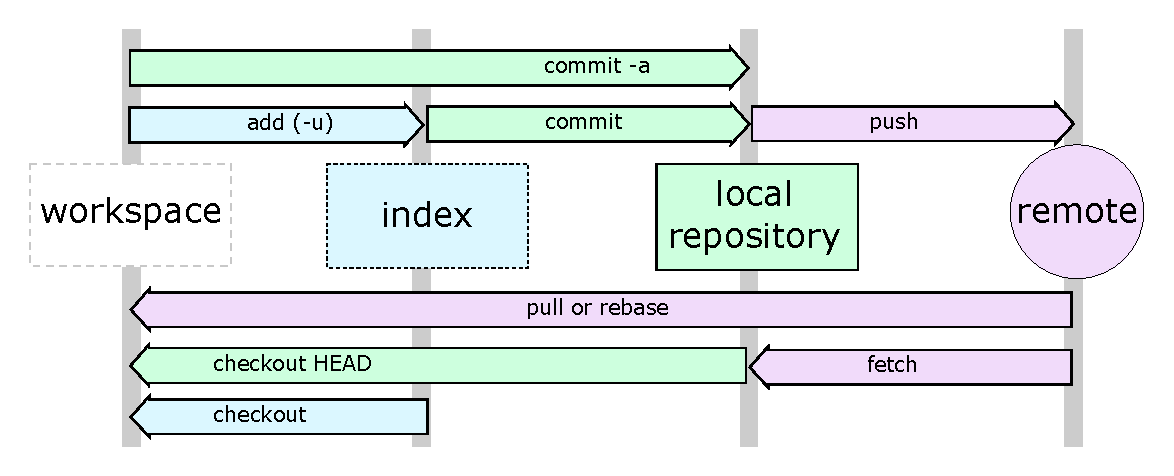
\includegraphics[
    width=\textwidth,
    height=\textheight,
    keepaspectratio
  ]{resources/git-workflow.pdf}
  \caption{Git-Workflow}
  \label{git-workflow}
\end{figure}
Die Grafik~\ref{git-workflow} stellt das Zusammenspiel der Artefakte und den Standard-Git-Worflow\footcite{osteele-git-workflow} dar.

\paragraph{Repositories} sind die größte Verwaltungseinheit in Git. Diese enthalten alle Git-Objekte, wie Referenzen, Commits, Trees, Blobs, sowie die lokale Konfiguration. Repositories können andere Repositories referenzieren oder referenziert werden, dabei können viele gängige Protokolle verwendet werden (http, ssh, ftp, absolute Pfade)

\paragraph{Commits} sind zeitlich determinierte, persönliche und kommentierte Referenzen auf einen konkreten Arbeitsstand (``Snapshot'') des Repositories. Ein Commit kann immer maximal nur auf einen Eltern-Commit verweisen, kann allerdings von beliebig vielen anderen Commits referenziert werden. Bei Betrachtung aller Commits, bilden dieser daher einen gerichteten Baumgraphen.

\paragraph{Branches} sind, im Gegensatz zu vielen anderen Versionverwaltungssystemen, in Git lediglich Verweise auf einen bestimmten Commit. Wenn ein Branch aktiv ist, dann wird mit jedem Commit auf diesem Branch, der Verweis auf den neuen Commit aktualisiert.

\paragraph{Tags} sind genauso wie Branches einfache Verweise auf einen Commit, allerdings verändert sich die Position eines Tags nach einem Commit nicht.

\paragraph{Remotes} sind Verweise in der Konfiguration eines Repositories auf andere Repositories. Dies wird im allgemeinen genutzt um Änderungen von dort zu holen oder dorthin zu bewegen. Es können beliebig viele Remotes für jedes Repository definiert werden. Zudem kann beliebig definiert werden, welche Branches von einem Repository Änderungen erhalten oder dieses aktualisieren.

\paragraph{Blobs} sind die komprimierten Inhalte einer Datei.

\paragraph{Trees} sind Referenzen von Blobs, und stellen damit im einfachsten Fall eine Ansicht eines Verzeichnisses und seiner Dateien dar.

\paragraph{Hashes} sind im allgemeinen Abbildung einer großen Abbildung von Zeichen auf eine deutlich geringere Menge. Die Abbildung führt immer zur gleichen Ergebnismenge. In Git werden Hashes als allgemeine Referenzierungsmöglichkeit verwendet. Alle Relationen werden darüber beschrieben und sind daher über alle Repositories gleich. Um die Eindeutigkeit 

\subsection{Interne Arbeitsweise}

Git verwendet intern einen Mix aus Referenzen, Indexierung, Komprimierung und Hashing. Zudem werden keine Differenzmengen, wie etwa in Subversion abgelegt, sondern immer vollständige Dateiinhalte. Diese Kombination bedeutet für viele Softwareprojekte eine deutliche Speicherplatzreduktion, wie zum Beispiel für das Mozilla-Projekt\footcite{kernel-git-svn}. Dadurch dass vollständig Dateiinhalte gesichert werden, ist Git für besonders große, schlecht zu komprimierende, sich häufig ändernde Dateien eher ungünstig. Für solche Dateien ist es sinnvoller 

Um die interne Arbeitsweise von Git zu erläutern, müssen die Zusammenhänge von Commits, Trees, Blobs und Hashes verdeutlicht werden.

Die Git-Objekte werden von Git immer anhand ihres Hashes abgelegt. Dabei wird ein 40-Stelliger SHA1-Hash verwendet. Die notwendigen Stellen zu Referenzierung sind aber häufig deutlich geringer, so können im allgemeinen Gebrauch deutlich verkürzte Zeichenketten verwendet werden. Im allgemeinen etwa 5 Stellen oder bei großen Projekten, wie dem Linux-Kernel, 12 Stellen.

Der Hash von Blobs ist eine Abbildung ihres Inhaltes. Daher werden Dateien mit den gleichen Inhalt auch immer auf den gleichen Blob abgebildet, unabhängig vom Verzeichnis in dem sie sich befinden oder wie oft sie geändert wurden.

Wie auch beim Blob sind Trees nur eine Abbildung ihres Inhaltes. Da Trees aber als eine Art Verzeichnis zu verstehen sind, referenzieren Trees andere Trees und Blobs. Damit würde eine Folge von Commits, die erste eine Datei erzeugt und schließlich wieder entfernt, am Ende wieder auf den gleichen Tree verweisen.

Commits schließlich verweisen auf einen oder mehrere Vorgänger-Commits, einen Tree, einen Autor und einen Commiter. Durch den Verweis auf den Vorgänger entsteht der in Darstellungen übliche Baum von Versionsknoten.

Dieser einfache, gut skalierbare Aufbau ermöglicht eine sehr leichtgewichtige Erstellung von Branches und damit zahlreiche flexible Arbeitsweisen.

\subsection{GitHub-Workflow}

GitHub ist heute die größte Plattformen für Quelloffene Softwareprojekte\footcite{github-marketshare-datanyze}. Durch die rasante Verbreitung von Git, wurde GitHub bei Open-Source-Projekten schnell zur Alternative für Sourceforge\footcite{heise-github-2011}. Damit einhergehend hatte der GitHub-Workflow\footcite{github-workflow-intro} auf die Git-Gemeinschaft hohen Einfluss.

Der GitHub-Workflow ist eine einfache Arbeitsweise, die auf Branches und manuellen Begutachtungen(Reviews) basiert. Änderungen gelangen nur zurück auf den Hauptstrang, wenn sie zuvor einem Review unterzogen worden. Dieser Schritt ist ein entscheidender Unterschied zum Trunk-Based-Workflow der mit Continuous-Integration propagiert wird, da hier der Code-Review erst nach der Integration mit dem Hauptzweig durchgeführt werden kann.

\subsection{Gitflow}

Gitflow ist ein weiterer bekannter Workflow mit Git\footcite{nvie-git-branch-model}. Im Gegensatz zum simplen GitHub-Workflow liegt beim Gitflow der Schwerpunkt auf der Erstellung eines Releases, also einer Menge an Commits, häufig auch von verschiedenen Autoren.

In Anlehnung an viele bekannte Modelle unterscheidet Gitflow zwischen Produktivzweig(master), außerplanmäßiger Anpassung(hotfix), Auslieferungszweig(release), Entwicklungszweig(development) und zahlreichen Feature- und Bug-Zweigen.

Gitflow unterscheidet wie viele andere Git-Arbeitsmodelle zwischen langlebigen und kurzlebigen Branches. Die langlebigen Branches sind hierbei ``master'' und ``development''. Alle anderen Branches sind kurzlebige Branches(``supporting branches''), die immer erst erstellt werden, wenn sie notwendig sind und gelöscht werden, sobald sie ihren Zweck erfüllt haben.

\begin{figure}[htbp]
  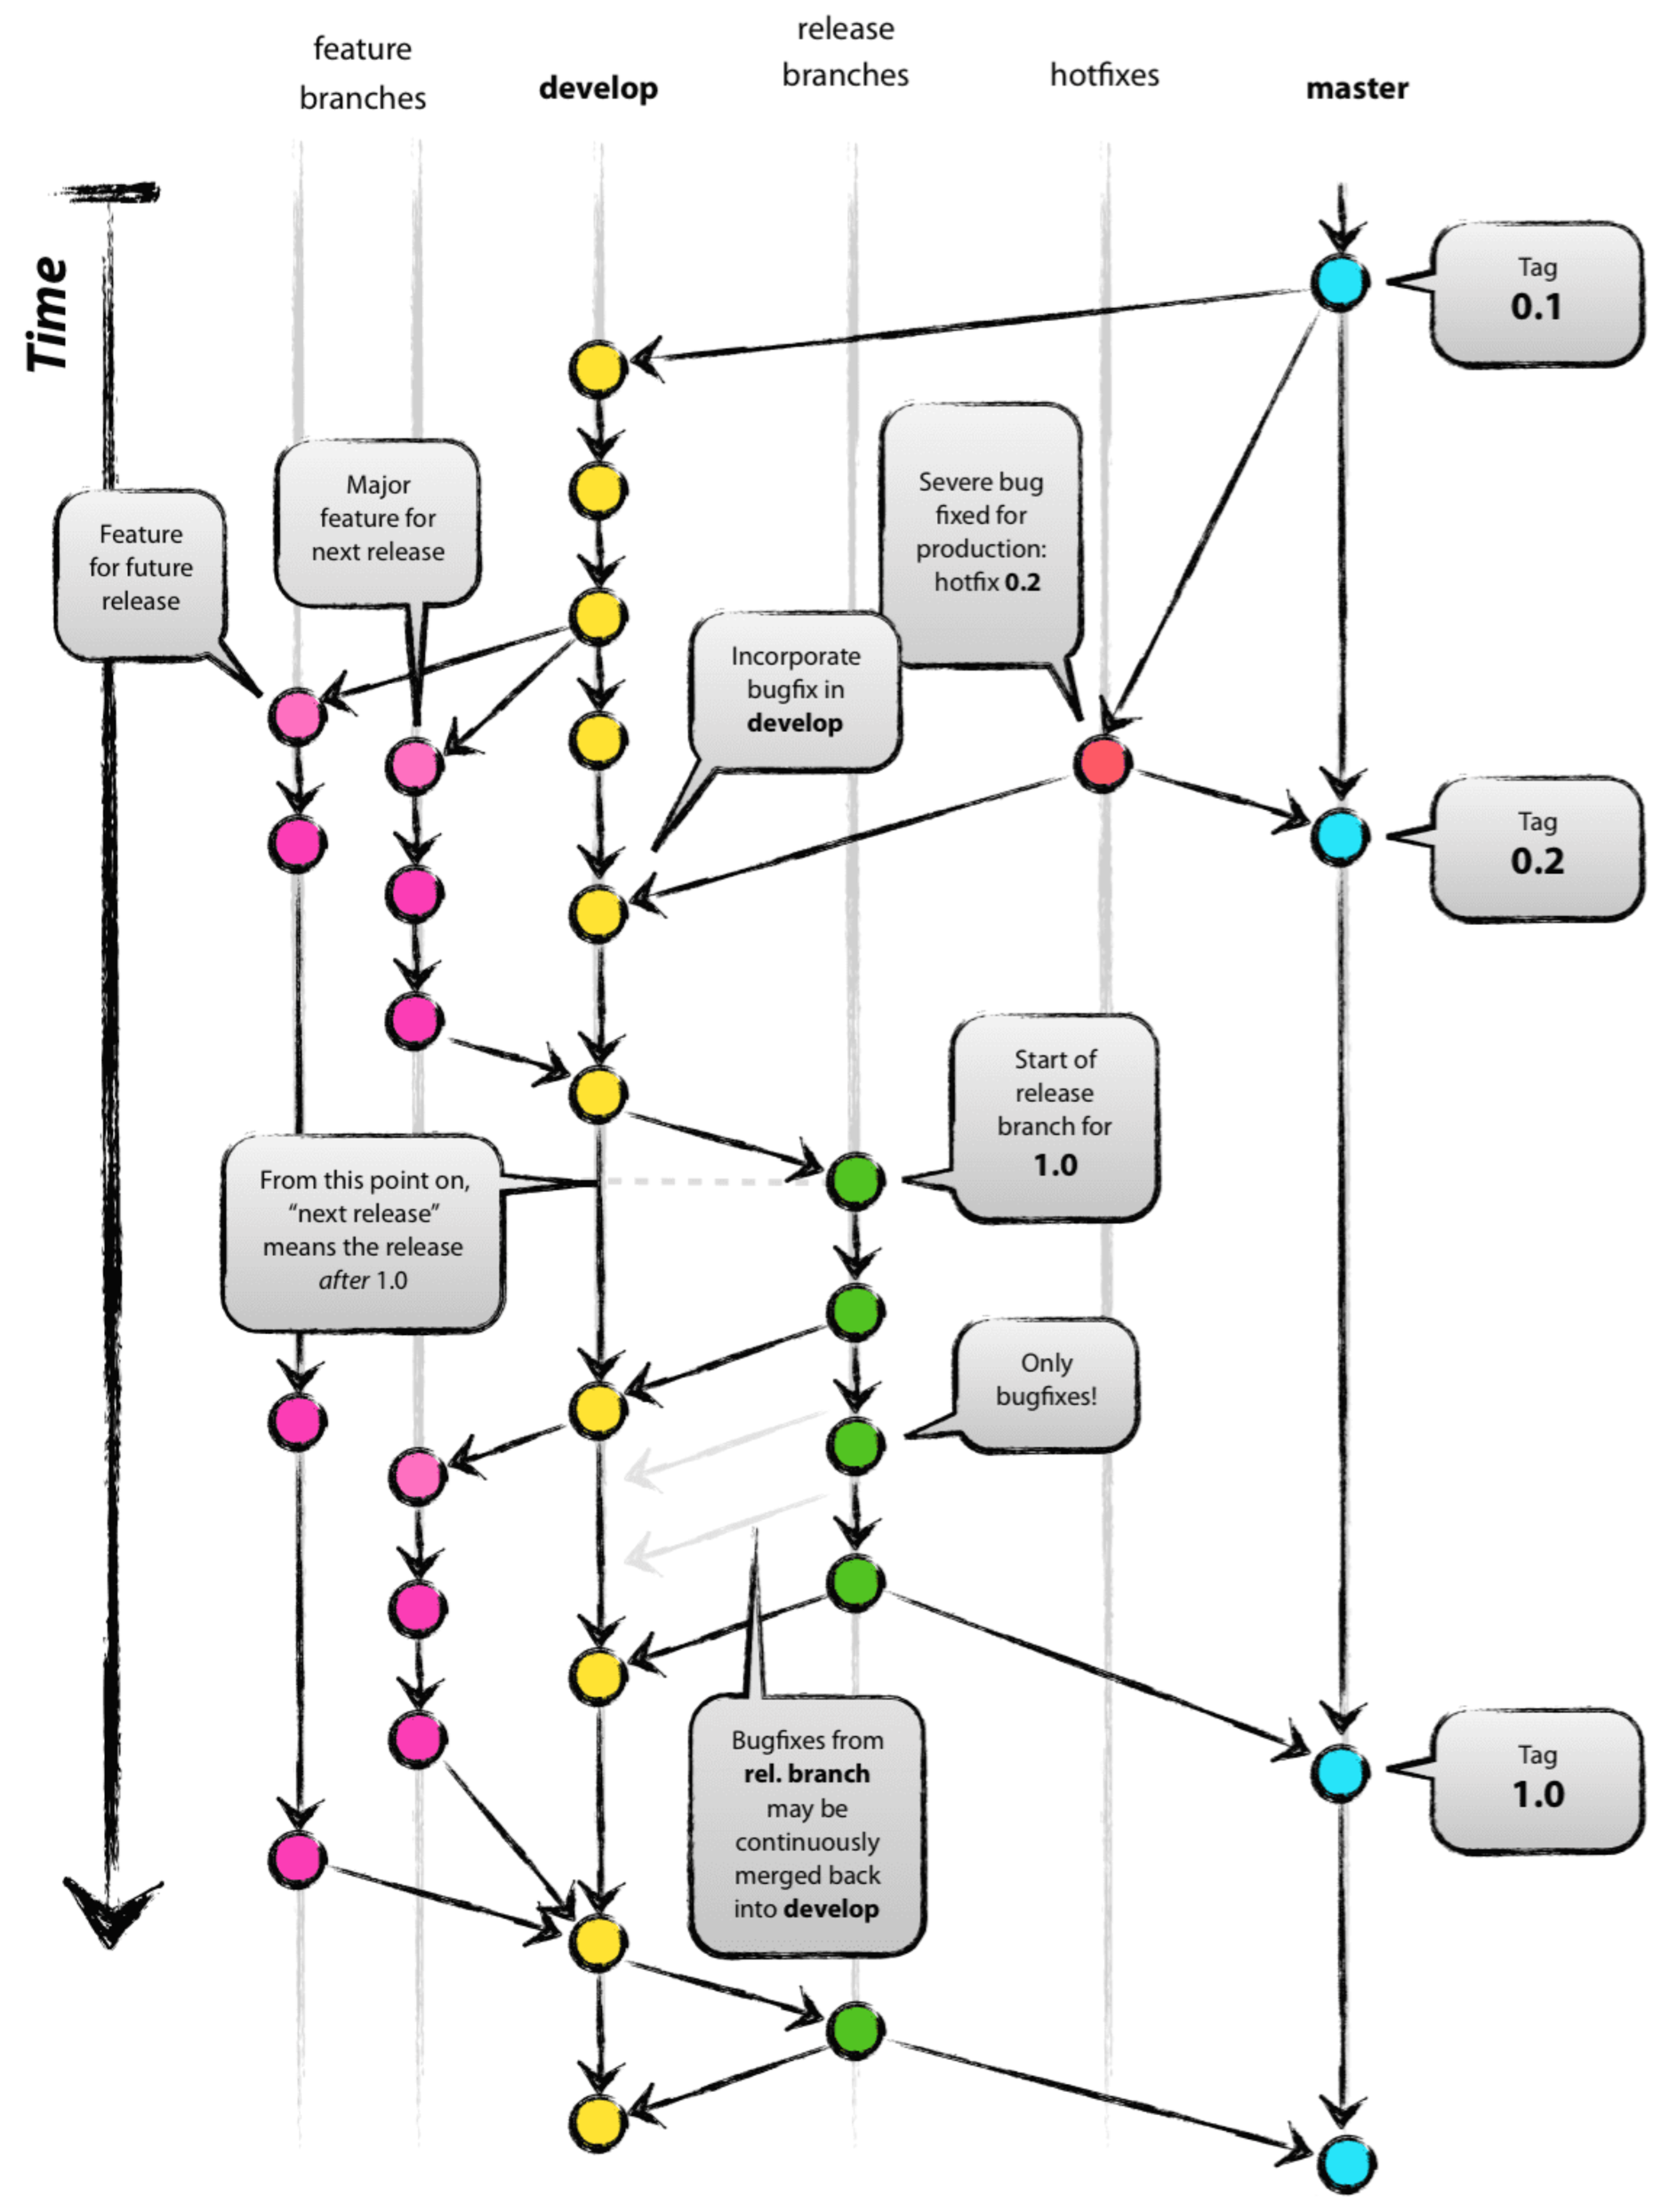
\includegraphics[
    width=\textwidth,
    height=\textheight,
    keepaspectratio
  ]{resources/git-flow.pdf}
  \caption{Gitflow-Workflow}
  \label{git-flow}
\end{figure}
Der konkrete Arbeitsfluss wird in der Abbildung~\ref{git-flow} zusammengefasst. Es wird deutlich dass nur Commits von Release- und Hotfix-Branches auf den Master-Branch gelangen können. Desweiteren ist herauszustellen, dass nach der Erstellung des Release-Branches keine Änderungen mehr vom Development-Branch zugeführt werden. Diese Trennung der Änderungsflüsse führt dazu, dass bereits an neuen Themen gearbeitet werden kann, ohne dass der Release behindert wird. Des Weiteren ist klar geregelt, dass alle Features immer erst im Development-Branch integriert werden müssen.

\section{Feature-Branches}

Die Idee hinter einem Feature Branch ist, dass für jedes neue Merkmal, beziehungsweise für jede neue Anforderung ein neuer Branch in der Versionsverwaltung erstellt wird. Ziel von Feature-Branches ist die Isolierung von Änderungen, um die anderen Zweige nicht zu blockieren und Änderungen erst nach Test und Abnahme zusammen zu führen. Dabei sollen mehrere Änderungen parallel entwickelt werden können, ohne dabei zu einem bestimmten Zeitpunkt alle Änderungen in einen Hauptzweig übernehmen zu müssen.

Prinzipiell ist diese Technik unabhängig von der verwendeten Versionsverwaltung, erhielt aber vor allem durch dezentrale Versionsverwaltungssysteme an Bedeutung. Der Grund dafür liegt in der deutlich einfacheren und weniger aufwändigen Erstellung von Branches und deren Zusammenführung.

Feature Branching wird kontrovers diskutiert[quote martinfowler feature branch, quote Yegor Bugayenko, quote jamesmckay]. Dabei wird angemahnt, dass die Abspaltung in einen Zweig, das Problem der Zusammenführung von Codeänderungen nicht behebt, sondern verschlimmert. So wird der Aufwand, der benötigt wird um zwei Verzweigungen zusammen zuführen, potentiell immer höher, um so mehr Änderungen hinzukommen. Die Aufwandserhöhung kann soweit gehen, dass ein psychologischer Faktor hinzukommt, der die Entscheidung zur Zusammenführung weiter belastet. Diese Zusammenführung wird dann auch als ``big scary merge'' oder ``big bang merge'' bezeichnet.

Kontrovers dazu wird die hervorgehoben, dass Feature-Branches Blockaden im Arbeitsfluss vermeiden und die Angst vor dem ``big scary merge'' durch Entwicklerdisziplin und Automatisierung gemildert. Entwicklerdisziplin meint hier Feature-Branches nur für kleine Änderungen zu verwenden und durch Hilfe von Automatisierung schnelle Rückmeldung über die Codequalität zu erhalten. Des Weiteren werden durch moderne ``pull based''[quote github about pull requests] Verzweigungsstratgien Entwickler dazu angehalten Codeprüfungen durch andere Entwickler einzufordern. Diese Lösungsstrategien werden in Kapitel~\ref{ch:visu_meth} weiterführend betrachtet.